\documentclass[11pt]{article}
\usepackage[
a4paper,
margin=1in,
headsep=4pt, % separation between header rule and text
]{geometry}
\usepackage{xcolor}
\usepackage{fancyhdr}
\usepackage{tgschola}
\usepackage{lastpage}
\usepackage[natbibapa]{apacite}
\usepackage{listings}
\usepackage{subfigure}
\usepackage{color}
\usepackage{dsfont}
\usepackage{footmisc}
\usepackage{verbatim}
\usepackage{smartdiagram}
\setlength{\marginparwidth}{0cm}
\setlength{\topmargin}{0cm}
\setlength{\voffset}{0cm}
\setlength{\headsep}{0cm}
\definecolor{dkgreen}{rgb}{0,0.6,0}
\definecolor{gray}{rgb}{0.5,0.5,0.5}
\definecolor{mauve}{rgb}{0.58,0,0.82}
\usepackage[utf8]{inputenc}
\graphicspath{{/Users/auddya/uw-me/2018/mechanicalBidomainModel/}}
\lstset{frame=tb,
	language=Java,
	aboveskip=3mm,
	belowskip=3mm,
	showstringspaces=false,
	columns=flexible,
	basicstyle={\small\ttfamily},
	numbers=none,
	numberstyle=\tiny\color{gray},
	keywordstyle=\color{blue},
	commentstyle=\color{dkgreen},
	stringstyle=\color{mauve},
	breaklines=true,
	breakatwhitespace=true,
	tabsize=3
}
\pagestyle{fancy}
\fancyhf{}
\fancyhead[C]{%
	\footnotesize\sffamily
	\yourname\quad
	web: \textcolor{blue}{\itshape\yourweb}\quad
	\textcolor{blue}{\youremail}}
\fancyfoot[C]{Page \thepage\ of \pageref{LastPage}}

\newcommand{\soptitle}{A computational study of mechanical bidomain model in durotaxis}

\newcommand{\yourname}{Debabrata Auddya}
\newcommand{\youremail}{auddya@wisc.edu}
\newcommand{\yourweb}{https://github.com/auddya}

\newcommand{\statement}[1]{\par\medskip
	\textcolor{blue}{\textbf{#1:}}\space
}

\usepackage[
breaklinks,
pdftitle={\yourname - \soptitle},
pdfauthor={\yourname},
unicode
]{hyperref}

\begin{document}
	
	\begin{center}
		\Large\soptitle
	\end{center}

\section*{Parameters}
N = 101 (No of nodes) \\
L = 0.005 m (Length of domain) \\
nu = 1000 Pa (Intracellular modulus) \\
mu\_zero = 1000 Pa (Extracellular modulus) \\
K = 50000000000 Pa/$m^{2}$ (Stiffness) \\
T =  200 Pa (Tension) \\
\section*{Code and Results}
\begin{lstlisting}
N = 101;
L = 0.005; %0.005m
g = 0; %100000; %100000 Pa/m
mu_zero = 1000; %1000 Pa
nu = 1000; %1000 Pa
K = 50000000000; %50GPa/m2
T = 200; %200Pa
w = zeros(N,1); %Extracellular displacement
u = zeros(N,1); %Intracellular displacement
x = zeros(N,1); %x position, useful when plotting
delta = (2*L)/(N-1); %Spacing along x direction
iterations = 100;
for i = 1:N
x(i) = L*(2*(i-1)/(N-1)-1); 
mu(i) = mu_zero + g*x(i);
end
for k = 1:iterations
for i = 2:(N-1)
a(i) = 4*mu(i)*(w(i+1)+w(i-1))+(mu(i+1)-mu(i-1))*(w(i+1)-w(i-1));
b(i) = 4*nu*(u(i+1)+u(i-1));
A(i) = 8*mu(i) + K*delta*delta;
C = 8*nu + K*delta*delta;
B = K*delta*delta;
u(i) = (a(i)*B + A(i)*b(i))/(A(i)*C - B*B);
w(i) = (a(i)/A(i)) + (B/A(i))*((a(i)*B + A(i)*b(i))/(A(i)*C - B*B));
end
%Apply Boundary Conditions
u(1) = u(2) + (T*delta/(4*nu));
w(1) = w(2);
u(N) = u(N-1) - (T*delta/(4*nu));
w(N) = w(N-1);
end 
for i = 1:N
h(i) = u(i)-w(i);
end 
plot(x,h)  %if you want plot with x in mm, use plot(x*1000,h)
xlabel('x');
ylabel('u-w');
title('Difference between extracellular and intracellular displacement');
\end{lstlisting}
\begin{figure}
	\begin{center}
		%
		\subfigure[Difference in displacements for g=0]{%
			\label{fig:uw0}
			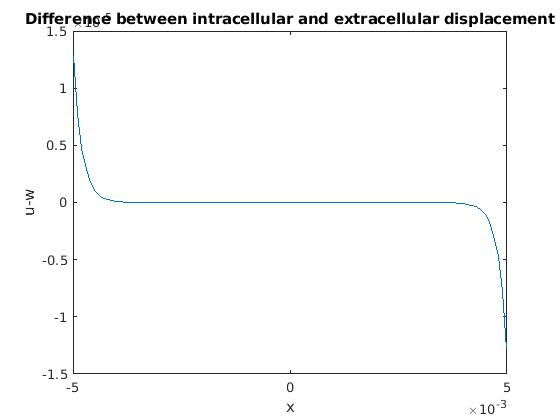
\includegraphics[width=0.4\textwidth]{/testResultsNew/u-w2(g_0).jpg}
		}%
		\subfigure[Difference in displacements for g=$10^5$]{%
			\label{fig:uwvar}
			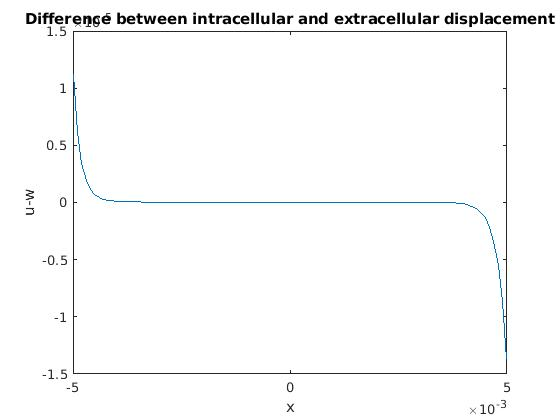
\includegraphics[width=0.4\textwidth]{/testResultsNew/u-w2(g_var).jpg}
		}\\ %  ------- End of the first row ----------------------%
		\subfigure[Intracellular displacement for g=0]{%
			\label{fig:u0}
			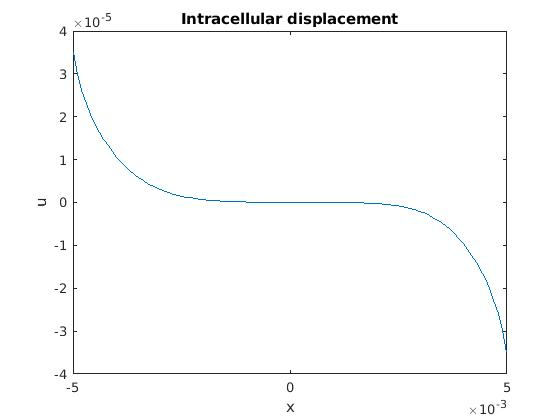
\includegraphics[width=0.4\textwidth]{/testResultsNew/u2(g_0).jpg}
		}%
		\subfigure[Intracellular displacement for g=$10^5$]{%
			\label{fig:uvar}
			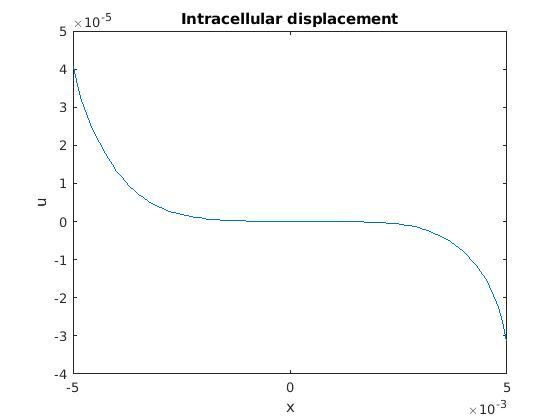
\includegraphics[width=0.4\textwidth]{/testResultsNew/u2(g_var).jpg}
		}\\
			\subfigure[Extracellular displacement for g=0]{%
		\label{fig:w0}
		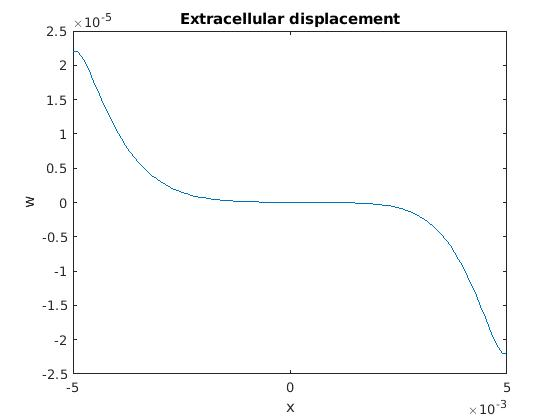
\includegraphics[width=0.4\textwidth]{/testResultsNew/w2(g_0).jpg}
	  }%
	\subfigure[Extracellular displacement for g=$10^5$]{%
		\label{fig:wvar}
		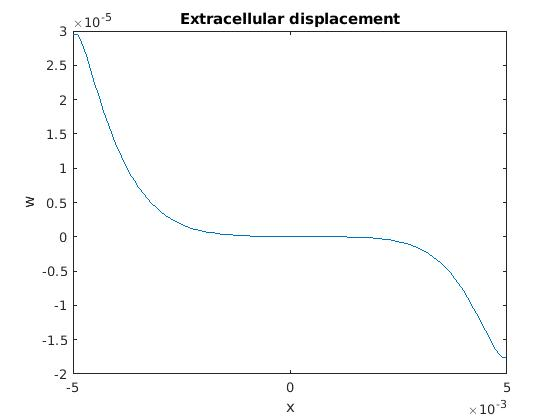
\includegraphics[width=0.4\textwidth]{/testResultsNew/w2(g_var).jpg}
	 }%
	\end{center}
	\caption{%
Comparison of results for g=0 and g=$10^5$ Pa/m (Iteration: 100). Elapsed time is 0.320051 seconds.
	}%
	\label{fig:subfigures2}
\end{figure}
\begin{figure}
	\begin{center}
		%
		\subfigure[Difference in displacements for g=0]{%
			\label{fig:uw02}
			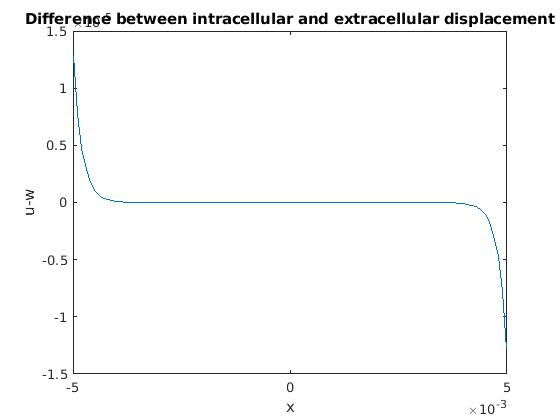
\includegraphics[width=0.4\textwidth]{/testResultsNew/u-w3(g_0).jpg}
		}%
		\subfigure[Difference in displacements for g=$10^5$]{%
			\label{fig:uwvar2}
			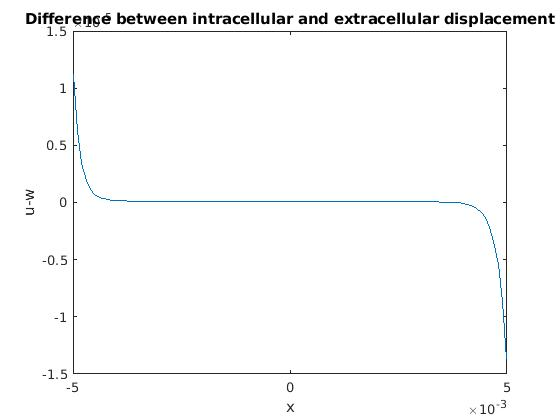
\includegraphics[width=0.4\textwidth]{/testResultsNew/u-w3(g_var).jpg}
		}\\ %  ------- End of the first row ----------------------%
		\subfigure[Intracellular displacement for g=0]{%
			\label{fig:u02}
			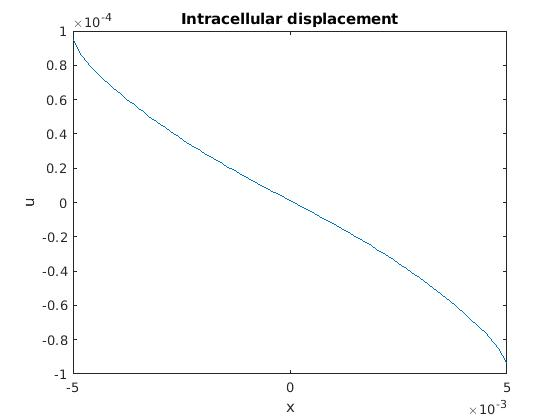
\includegraphics[width=0.4\textwidth]{/testResultsNew/u3(g_0).jpg}
		}%
		\subfigure[Intracellular displacement for g=$10^5$]{%
			\label{fig:uvar3}
			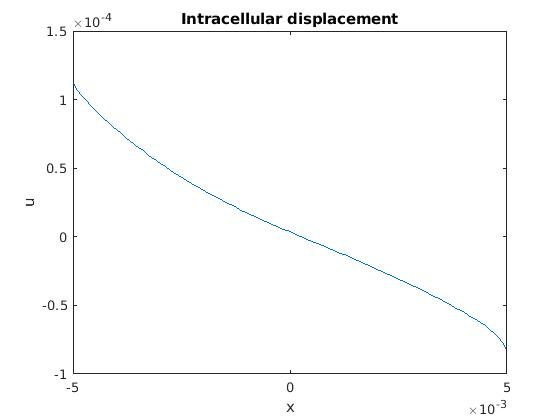
\includegraphics[width=0.4\textwidth]{/testResultsNew/u3(g_var).jpg}
		}\\
		\subfigure[Extracellular displacement for g=0]{%
			\label{fig:w03}
			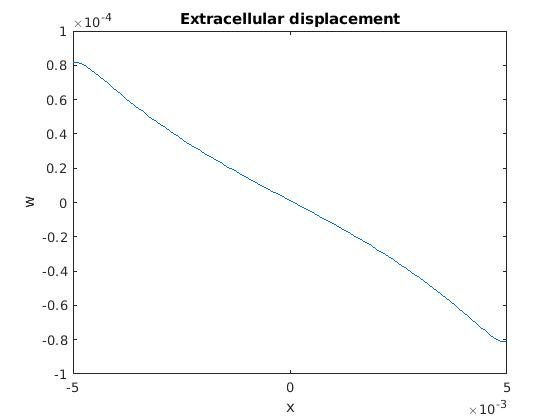
\includegraphics[width=0.4\textwidth]{/testResultsNew/w3(g_0).jpg}
		}%
		\subfigure[Extracellular displacement for g=$10^5$]{%
			\label{fig:wvar3}
			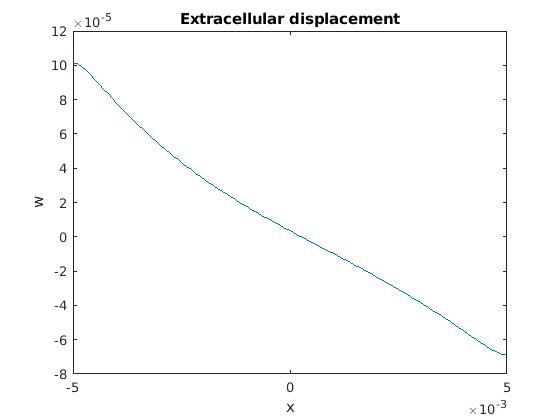
\includegraphics[width=0.4\textwidth]{/testResultsNew/w3(g_var).jpg}
		}%
	\end{center}
	\caption{%
		Comparison of results for g=0 and g=$10^5$ Pa/m (Iteration: 1000). Elapsed time is 0.366209 seconds.
	}%
	\label{fig:subfigures3}
\end{figure}
\begin{figure}
	\begin{center}
		%
		\subfigure[Difference in displacements for g=0]{%
			\label{fig:uw04}
			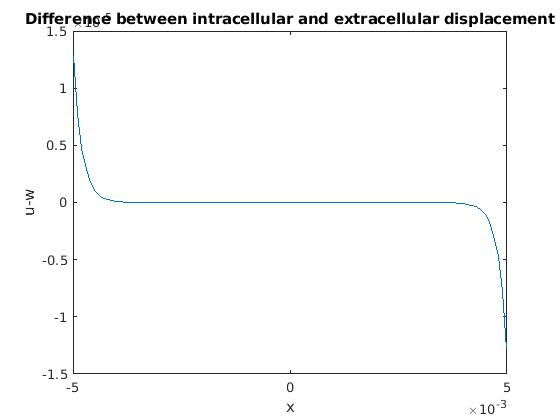
\includegraphics[width=0.4\textwidth]{/testResultsNew/u-w4(g_0).jpg}
		}%
		\subfigure[Difference in displacements for g=$10^5$]{%
			\label{fig:uwvar4}
			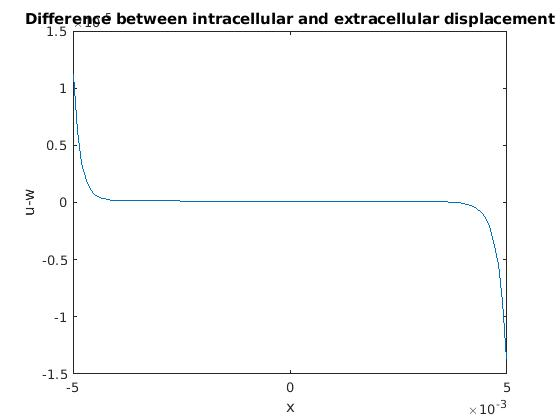
\includegraphics[width=0.4\textwidth]{/testResultsNew/u-w4(g_var).jpg}
		}\\ %  ------- End of the first row ----------------------%
		\subfigure[Intracellular displacement for g=0]{%
			\label{fig:u04}
			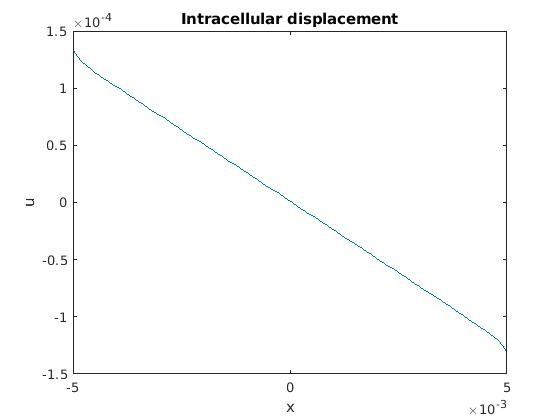
\includegraphics[width=0.4\textwidth]{/testResultsNew/u4(g_0).jpg}
		}%
		\subfigure[Intracellular displacement for g=$10^5$]{%
			\label{fig:uvar4}
			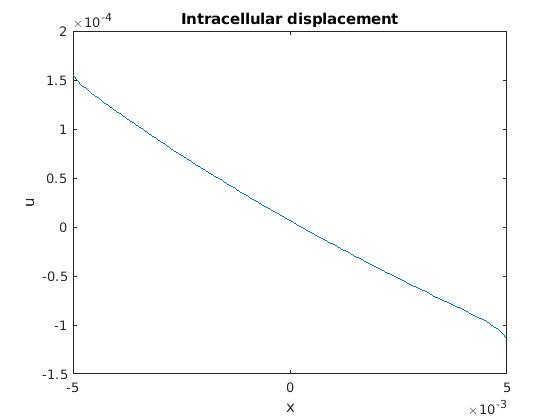
\includegraphics[width=0.4\textwidth]{/testResultsNew/u4(g_var).jpg}
		}\\
		\subfigure[Extracellular displacement for g=0]{%
			\label{fig:w04}
			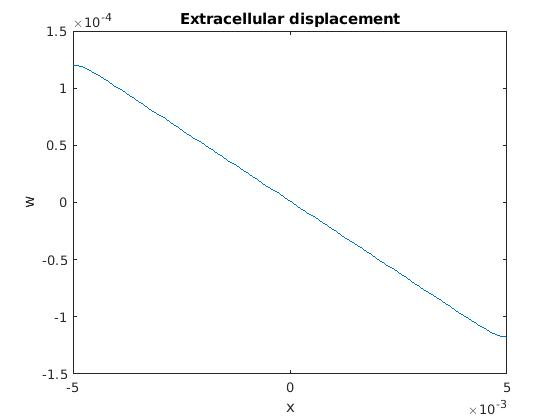
\includegraphics[width=0.4\textwidth]{/testResultsNew/w4(g_0).jpg}
		}%
		\subfigure[Extracellular displacement for g=$10^5$]{%
			\label{fig:wvar4}
			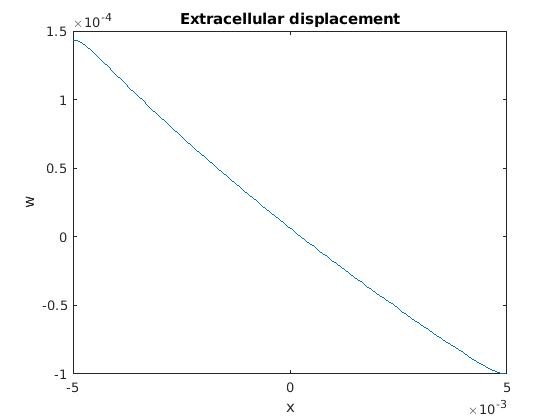
\includegraphics[width=0.4\textwidth]{/testResultsNew/w4(g_var).jpg}
		}%
	\end{center}
	\caption{%
		Comparison of results for g=0 and g=$10^5$ Pa/m (Iteration: 10000). Elapsed time is 0.414921 seconds.
	}%
	\label{fig:subfigures4}
\end{figure}
\begin{figure}
	\begin{center}
		%
		\subfigure[Difference in displacements for g=0]{%
			\label{fig:uw05}
			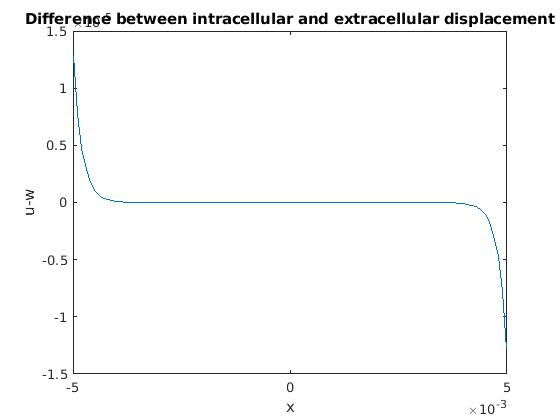
\includegraphics[width=0.4\textwidth]{/testResultsNew/u-w5(g_0).jpg}
		}%
		\subfigure[Difference in displacements for g=$10^5$]{%
			\label{fig:uwvar5}
			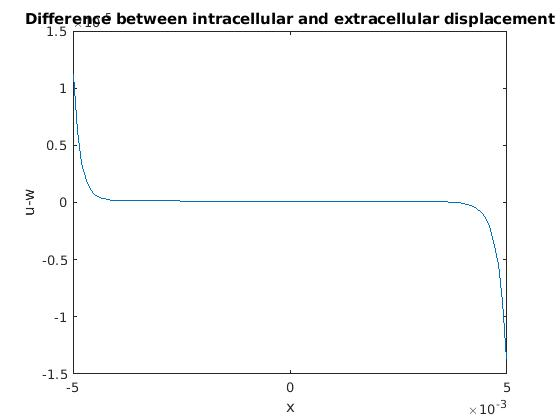
\includegraphics[width=0.4\textwidth]{/testResultsNew/u-w5(g_var).jpg}
		}\\ %  ------- End of the first row ----------------------%
		\subfigure[Intracellular displacement for g=0]{%
			\label{fig:u05}
			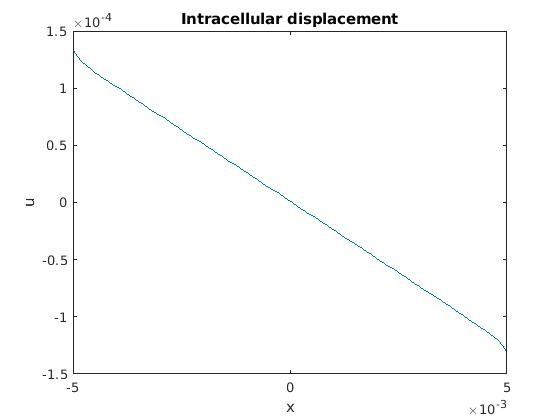
\includegraphics[width=0.4\textwidth]{/testResultsNew/u5(g_0).jpg}
		}%
		\subfigure[Intracellular displacement for g=$10^5$]{%
			\label{fig:uvar5}
			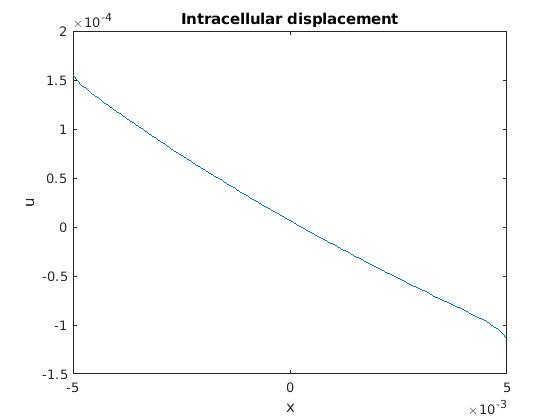
\includegraphics[width=0.4\textwidth]{/testResultsNew/u5(g_var).jpg}
		}\\
		\subfigure[Extracellular displacement for g=0]{%
			\label{fig:w05}
			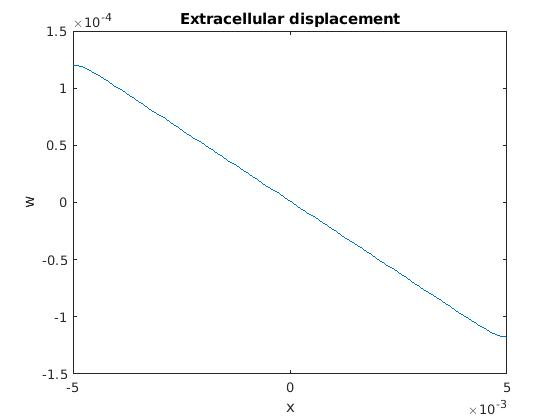
\includegraphics[width=0.4\textwidth]{/testResultsNew/w5(g_0).jpg}
		}%
		\subfigure[Extracellular displacement for g=$10^5$]{%
			\label{fig:wvar5}
			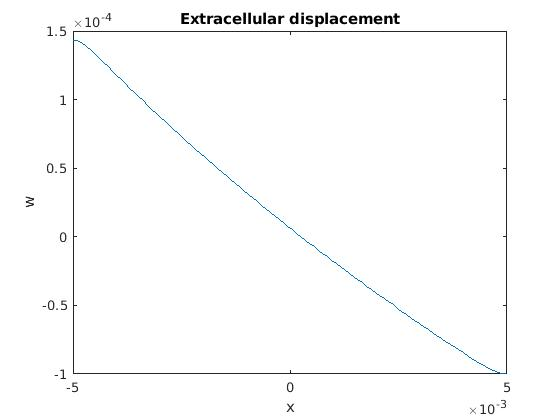
\includegraphics[width=0.4\textwidth]{/testResultsNew/w5(g_var).jpg}
		}%
	\end{center}
	\caption{%
		Comparison of results for g=0 and g=$10^5$ Pa/m (Iteration: 100000). Elapsed time is 0.772543 seconds.
	}%
	\label{fig:subfigures5}
\end{figure}
\begin{figure}
	\begin{center}
		%
		\subfigure[Difference in displacements for g=0]{%
			\label{fig:uw06}
			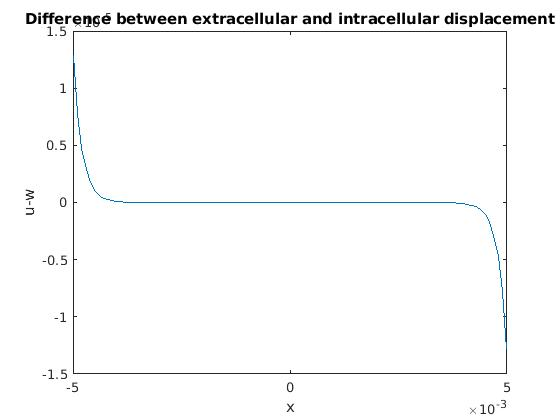
\includegraphics[width=0.4\textwidth]{/testResultsNew/u-w6(g_0).jpg}
		}%
		\subfigure[Difference in displacements for g=$10^5$]{%
			\label{fig:uwvar6}
			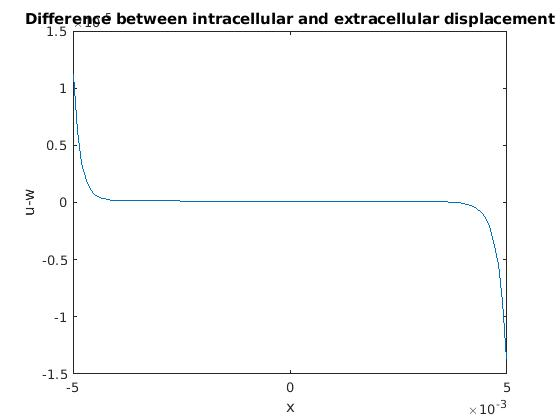
\includegraphics[width=0.4\textwidth]{/testResultsNew/u-w6(g_var).jpg}
		}\\ %  ------- End of the first row ----------------------%
		\subfigure[Intracellular displacement for g=0]{%
			\label{fig:u06}
			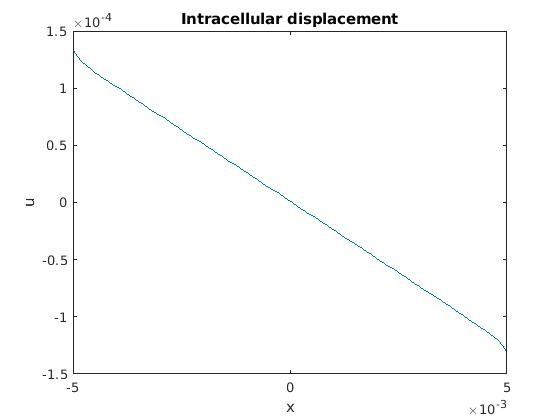
\includegraphics[width=0.4\textwidth]{/testResultsNew/u6(g_0).jpg}
		}%
		\subfigure[Intracellular displacement for g=$10^5$]{%
			\label{fig:uvar6}
			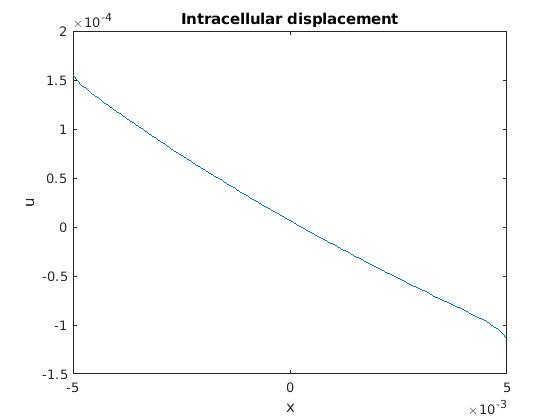
\includegraphics[width=0.4\textwidth]{/testResultsNew/u6(g_var).jpg}
		}\\
		\subfigure[Extracellular displacement for g=0]{%
			\label{fig:w06}
			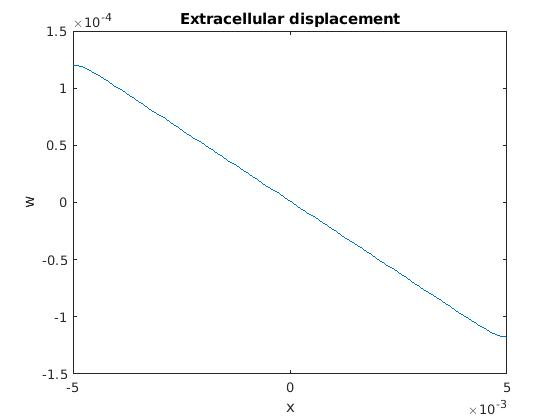
\includegraphics[width=0.4\textwidth]{/testResultsNew/w6(g_0).jpg}
		}%
		\subfigure[Extracellular displacement for g=$10^5$]{%
			\label{fig:wvar6}
			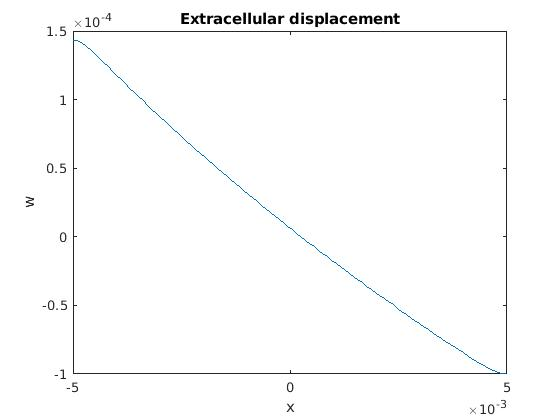
\includegraphics[width=0.4\textwidth]{/testResultsNew/w6(g_var).jpg}
		}%
	\end{center}
	\caption{%
		Comparison of results for g=0 and g=$10^5$ Pa/m (Iteration: 1000000). Elapsed time is 6.259795 seconds.
	}%
	\label{fig:subfigures6}
\end{figure}
\section*{Difference of displacements as a function of stiffness gradient}
\begin{figure}[htb]
  \begin{center}
 	 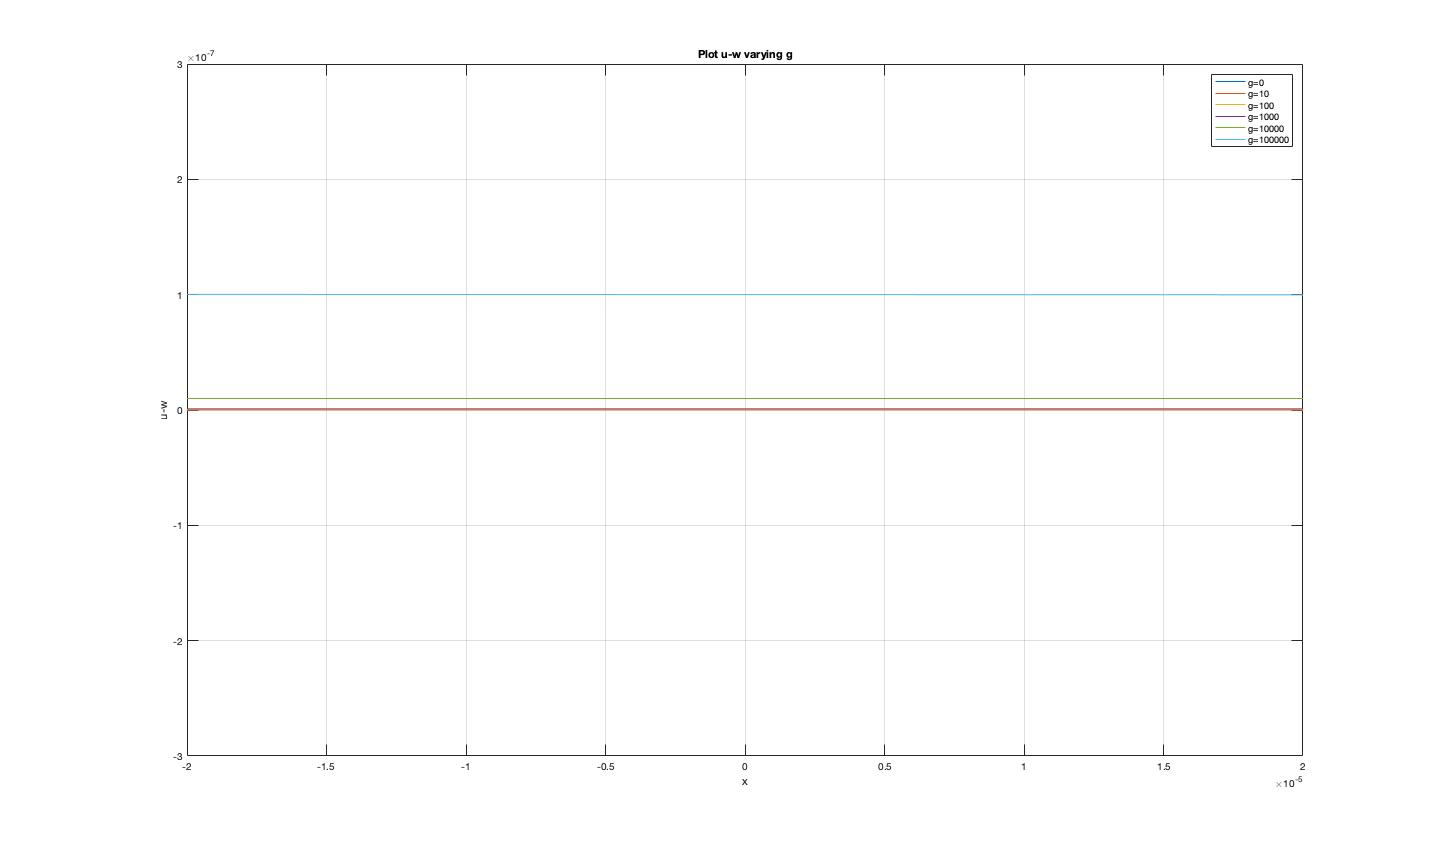
\includegraphics[scale=0.3]{/testResultsNew/variationG.jpg}
	\caption{Difference in intracellular and extracellular displacements about x = 0 as a function of \textbf{g}}
	\label{fig:uwG}
 \end{center}
\end{figure}
\newpage
\section*{Over Relaxation}
Variation of computation time with linearly increasing over relaxation parameter. The \textbf{stars} indicate the minimum value in each iteration limit. The figures below illustrate with iteration ranges from $10^2$ to $10^4$ 
\begin{figure}[htb]
  \begin{center}
	 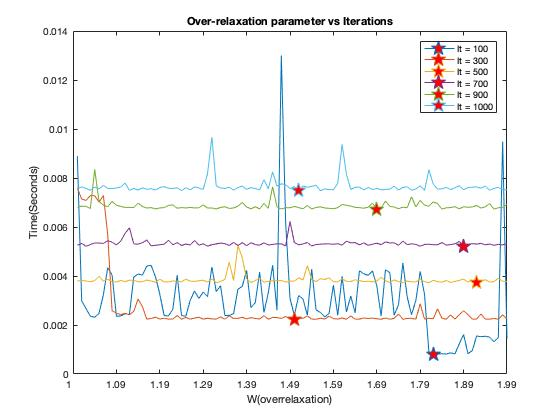
\includegraphics[scale = 0.85]{/testResultsNew/ite2.jpg}
	 \caption{Iteration range: 100 - 1000}
	 \label{fig:ite2}
  \end{center}
\end{figure}
\begin{figure}[htb]
  \begin{center}
	 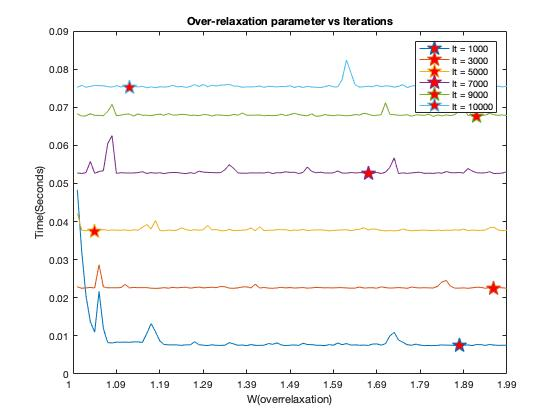
\includegraphics[scale = 0.85]{/testResultsNew/ite3.jpg}
	 \caption{Iteration range: 1000 - 10000}
	 \label{fig:ite3}
  \end{center}
\end{figure}
\begin{figure}[htb]
  \begin{center}
	 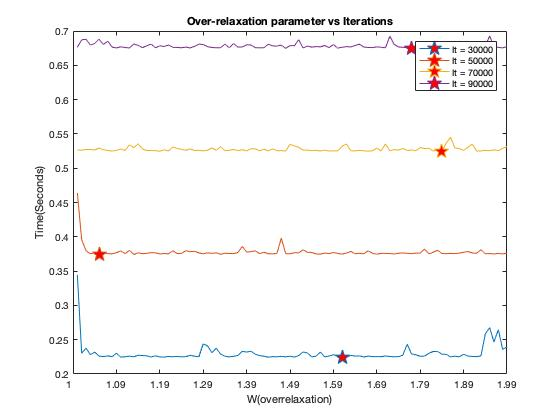
\includegraphics[scale = 0.85]{/testResultsNew/ite4.jpg}
	 \caption{Iteration range: 30000 - 90000}
	 \label{fig:ite4}
  \end{center}
\end{figure}
%\newpage
%\section*{SOR Iterations against time}
%\begin{table}[htb]
%	\centering
%	\resizebox{\textwidth}{!}{%
%		\begin{tabular}{lll}
%			Iterations & Time (seconds) & Relaxation Value \\
%			100        & 0.000535       & 1.94             \\
%			1000       & 0.0055         & 1.87             \\
%			10000      & 0.0541         & 1.95             \\
%			100000     & 0.5556         & 1.92             \\
%			1000000    & 5.4486         & 1.91            
%		\end{tabular}%
%	}
%\end{table}
\end{document}
